\documentclass[11pt]{article}

% ---------- Paquetes ----------
\usepackage[spanish,es-noshorthands]{babel}
\usepackage[utf8]{inputenc}
\usepackage[T1]{fontenc}
\usepackage[margin=2.5cm]{geometry}
\usepackage{graphicx}
\usepackage{booktabs}
\usepackage{longtable}
\usepackage{array}
\usepackage{caption}
\usepackage{float}
\usepackage{xcolor}
\usepackage[colorlinks=true, linkcolor=black, citecolor=black, urlcolor=blue]{hyperref}
\usepackage{parskip}
\usepackage{fancyhdr}
\usepackage{amsmath}
\usepackage{amssymb}

% Todas las imagenes viven en img/, junto a este .tex, dentro de docs/
\graphicspath{{img/}}
\setlength{\headheight}{14pt}
\setlength{\parindent}{0pt}
\setlength{\parskip}{6pt}

\pagestyle{fancy}
\fancyhf{}
\fancyhead[L]{Laboratorio 4, Parte 2 -- Modelos con Datos Geoespaciales}
\fancyhead[R]{CC3084 -- Data Science}
\fancyfoot[C]{\thepage}
\renewcommand{\headrulewidth}{0.4pt}

\title{\vspace{-1.5cm}\textbf{Detección de cianobacteria en los lagos de Atitlán y Amatitlán mediante Machine Learning}\\
\large Parte 2: Clasificación, validación espacio-temporal e interpretabilidad}
\author{
  Javier España \#23361 \and
  Ángel Esquit \#23221 \and
  Roberto Barreda \#23354
}
\date{Universidad del Valle de Guatemala \\ Facultad de Ingeniería -- CC3084 Data Science \\ Semestre II, 2026}

\begin{document}

\maketitle
\thispagestyle{empty}

\begin{abstract}
\noindent En la Parte I de este laboratorio se construyó, a partir de 22 imágenes Sentinel-2 (11 fechas por lago, enero 2025 -- julio 2026), un índice de cianobacteria (clorofila-\(a\) vía NDCI) para los lagos de Atitlán y Amatitlán. En esta segunda parte se usa ese mismo índice para entrenar modelos de Machine Learning capaces de clasificar, píxel por píxel, zonas de alta presencia de cianobacteria a partir de bandas espectrales, índices derivados y características geográficas. Se construyó un conjunto de 3{,}321{,}327 observaciones válidas, se entrenaron y compararon tres clasificadores (Regresión Logística, Random Forest y XGBoost), y se evaluaron bajo tres estrategias de validación: aleatoria, espacial (bloques de 1 km) y temporal (por fecha). El hallazgo principal no es qué modelo es mejor, sino que \textbf{la estrategia de validación pesa más que el modelo elegido}: el F1-Score de XGBoost se mueve entre 0.31 (transferencia entre lagos) y 0.89 (división aleatoria) según cómo se mida, un rango mucho mayor que la diferencia entre los tres algoritmos bajo una misma validación. El modelo generaliza bien dentro de Amatitlán, con reservas en Atitlán por su extremo desbalance de clases, pero no se transfiere de un lago al otro sin datos etiquetados de ese lago, y pierde desempeño de forma notable cuando se le pide predecir fechas futuras en vez de zonas nuevas.
\end{abstract}

\tableofcontents

% ======================================================================
\section{Introducción}
% ======================================================================

La Parte I de este laboratorio documentó que Amatitlán atraviesa una eutrofización crónica (clorofila-\(a\) media de 18.4 mg/m\(^3\), con un evento de floración total en junio de 2026 que cubrió el 76.6\,\% de su superficie) mientras que Atitlán se mantiene saludable a nivel de lago completo, con focos puntuales de floración cerca de algunas bahías. Esta segunda parte retoma esos mismos datos, pero cambia la pregunta: en lugar de describir qué pasó, se busca \textbf{predecir} qué zonas de un lago tienen alta probabilidad de presentar cianobacteria a partir de las bandas espectrales, sin necesitar primero calcular el índice de clorofila.

Esto tiene valor práctico porque el índice de clorofila-\(a\) que se usa como referencia (v\'ia NDCI) es en sí mismo una fórmula de calibración empírica, no una medición directa. Un modelo de clasificación entrenado sobre esos datos puede, en principio, generalizar el patrón espectral de la floración a datos nuevos, y sus variables de mayor peso pueden dar pistas físicas sobre qué es lo que realmente distingue una zona en floración de una que no lo está.

El resto del informe sigue la estructura de los diez ejercicios del enunciado: preparación del dataset (Sección~\ref{sec:datos}), construcción de la variable respuesta (Sección~\ref{sec:respuesta}), selección de predictores (Sección~\ref{sec:predictores}), entrenamiento de los tres modelos (Sección~\ref{sec:modelos}), su evaluación (Sección~\ref{sec:evaluacion}), validación espacial y temporal (Sección~\ref{sec:validacion}), generalización entre lagos (Sección~\ref{sec:generalizacion}), interpretabilidad (Sección~\ref{sec:interpretabilidad}), mapas predictivos (Sección~\ref{sec:mapas}) y conclusiones (Sección~\ref{sec:conclusiones}). El detalle técnico completo, con el código en Python, está en el notebook \texttt{Lab4\_Parte2\_ML.ipynb} del repositorio del proyecto.

% ======================================================================
\section{Preparación de los datos para Machine Learning}
\label{sec:datos}
% ======================================================================

\subsection{Construcción del conjunto de datos georreferenciado}

A diferencia de la Parte I, donde cada fecha se resumía en un promedio por lago, aquí cada observación es un \textbf{píxel individual} de 20 por 20 metros dentro del espejo de agua estable de cada lago (la misma huella morfológica calculada en la Parte I). Por cada píxel válido, en cada una de las fechas disponibles, se registró:

\begin{itemize}
    \item Coordenadas proyectadas (\texttt{x\_utm}, \texttt{y\_utm} en EPSG:32615) y geográficas (\texttt{lon}, \texttt{lat} en WGS 84).
    \item Fecha de la toma y lago al que pertenece.
    \item Reflectancia de las 9 bandas espectrales usadas en la Parte I: \texttt{B02}, \texttt{B03}, \texttt{B04}, \texttt{B05}, \texttt{B07}, \texttt{B08}, \texttt{B8A}, \texttt{B11}, \texttt{B12}.
    \item Índices derivados: NDVI, NDWI, NDCI, clorofila-\(a\) (Chl-\(a\)) y FAI, calculados con las mismas fórmulas de la Parte I para que ambas partes sean comparables.
    \item Distancia a la orilla en metros (\texttt{distancia\_orilla\_m}), calculada con una transformada de distancia euclidiana sobre la huella de agua.
\end{itemize}

\subsection{Control de calidad y eliminación de observaciones no válidas}

Se aplicaron tres filtros, en este orden:

\begin{enumerate}
    \item \textbf{Límites del lago.} Solo se conservan píxeles dentro de la huella de agua estable (\texttt{*\_huella.npz} de la Parte I); quedan fuera la tierra y las orillas secas.
    \item \textbf{Píxeles sin dato.} Se eliminan los píxeles marcados como \texttt{NoData}, con reflectancia en cero, o donde el NDCI no es evaluable (reflectancia \(\le 0\) en \texttt{B04} o \texttt{B05}), algo frecuente en las laderas sombreadas de la caldera de Atitlán.
    \item \textbf{Fechas poco confiables.} Se descartan las fechas con menos de 70\,\% de cobertura válida dentro de la huella (columna \texttt{Confiable} de \texttt{indices\_<lago>.csv}, calculada en la Parte I). El único caso es Atitlán 2025-01-18, con apenas 23\,\% de huella utilizable.
\end{enumerate}

Tras estos filtros quedaron \textbf{3{,}321{,}327 observaciones válidas}: 2{,}942{,}535 en Atitlán y 378{,}792 en Amatitlán, repartidas en 19 fechas distintas (10 de Atitlán y 10 de Amatitlán; ambos lagos comparten dos fechas, 2026-04-13 y 2026-04-28). El porcentaje de valores faltantes es prácticamente nulo para todas las variables (0\,\% en bandas y coordenadas, 0.115\,\% en NDVI por divisiones indeterminadas puntuales).

\subsection{Análisis exploratorio}

La Figura~\ref{fig:eda} muestra la distribución de clorofila-\(a\), NDCI, NDVI, NDWI, FAI y distancia a la orilla para ambos lagos. Amatitlán exhibe una cola mucho más larga hacia valores altos de clorofila-\(a\), consistente con su régimen eutrófico ya documentado en la Parte I.

\begin{figure}[H]
    \centering
    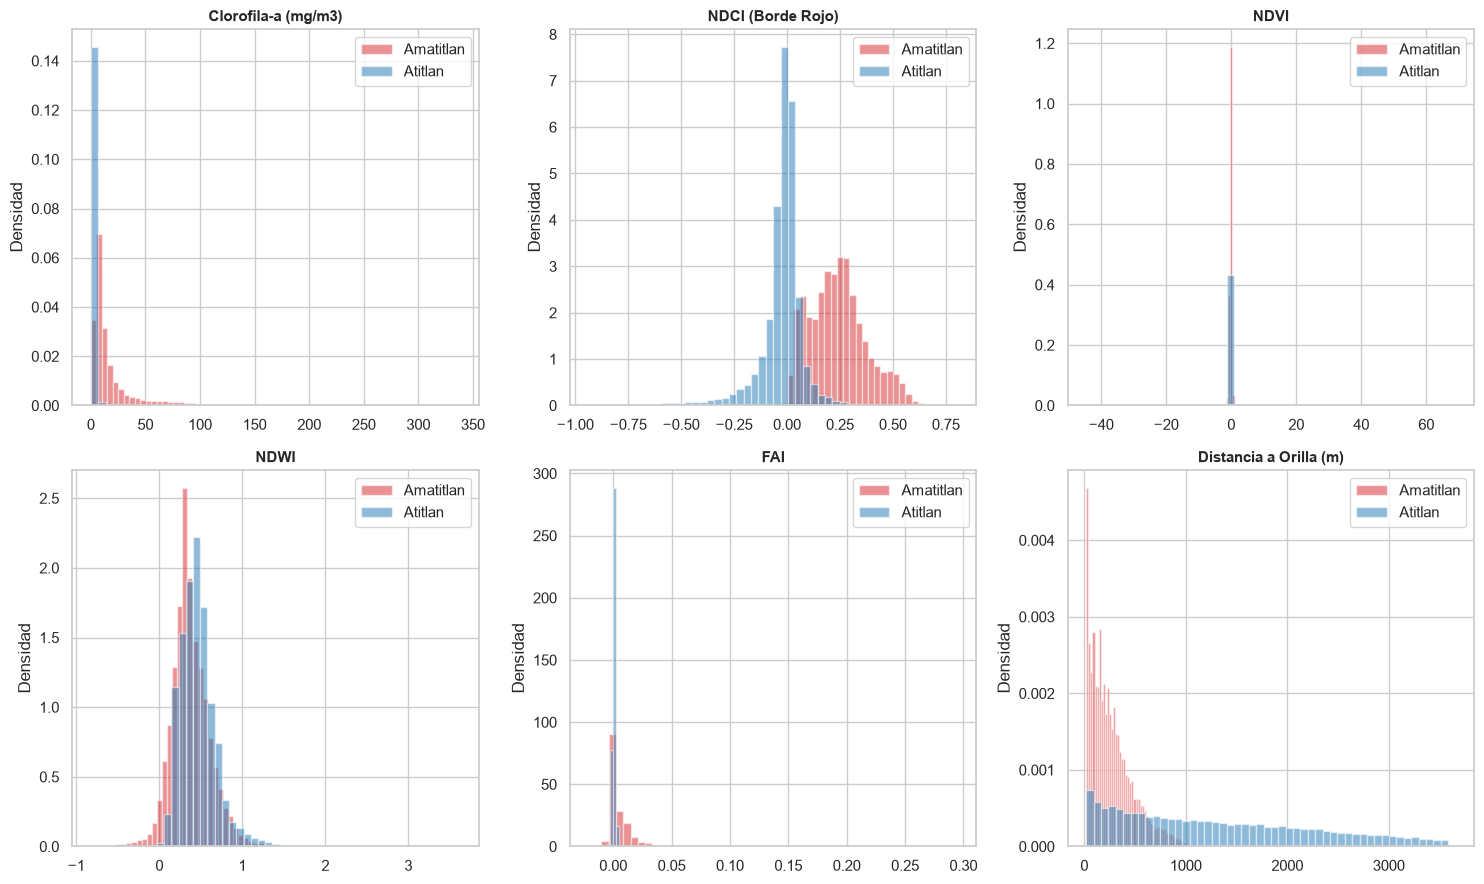
\includegraphics[width=0.95\textwidth]{eda_distribuciones.png}
    \caption{Distribución de las variables espectrales y derivadas por lago (muestra de hasta 50{,}000 píxeles por lago para agilizar el gráfico).}
    \label{fig:eda}
\end{figure}

\begin{figure}[H]
    \centering
    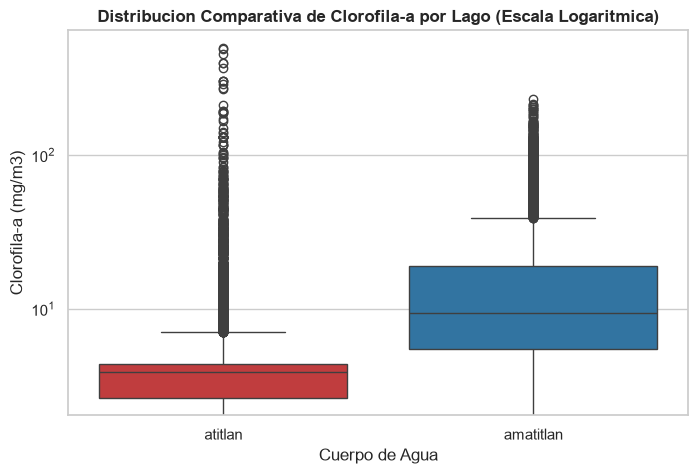
\includegraphics[width=0.65\textwidth]{boxplot_chla_lago.png}
    \caption{Distribución comparativa de clorofila-\(a\) por lago, en escala logarítmica (muestra de 100{,}000 píxeles).}
    \label{fig:boxplot_chla}
\end{figure}

La Figura~\ref{fig:correlacion} muestra la matriz de correlación entre las 9 bandas y los 5 índices derivados. Las bandas espectrales están, como es de esperar, fuertemente correlacionadas entre sí (todas responden en mayor o menor grado a la misma reflectancia superficial), mientras que NDCI y Chl-\(a\) se comportan como un bloque casi independiente del resto.

\begin{figure}[H]
    \centering
    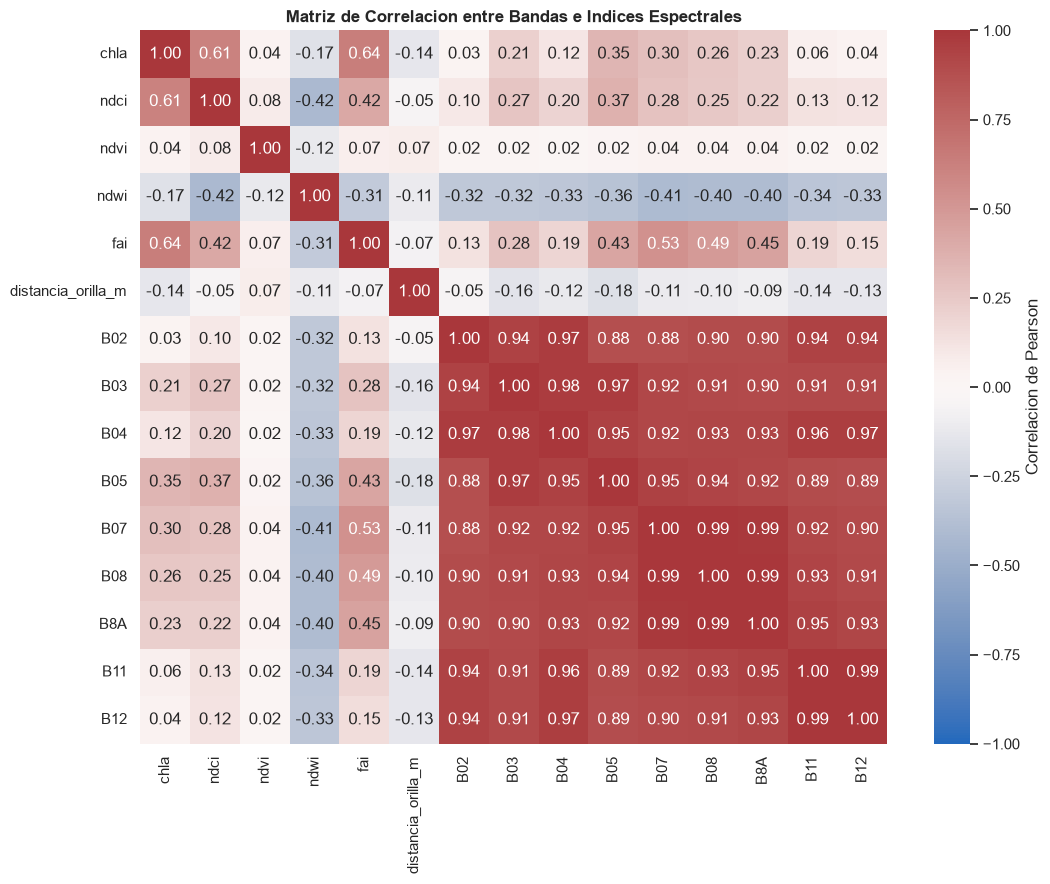
\includegraphics[width=0.85\textwidth]{correlacion_bandas_indices.png}
    \caption{Matriz de correlación de Pearson entre bandas espectrales e índices derivados (muestra de 100{,}000 píxeles).}
    \label{fig:correlacion}
\end{figure}

\subsection{Decisiones de preparación y limpieza}

\begin{enumerate}
    \item \textbf{Huella de agua estable en lugar de máscara por fecha.} Una máscara de agua calculada fecha por fecha cambiaría de tamaño con la nubosidad y el oleaje, y el área analizada dejaría de ser comparable entre imágenes.
    \item \textbf{Eliminación de sombras y ceros de reflectancia} (\(B04 \le 0\) o \(B05 \le 0\)), frecuentes en las laderas de la caldera de Atitlán, que harían indeterminado el cociente del NDCI.
    \item \textbf{Descarte de escenas con menos de 70\,\% de cobertura.} Con tan poca área visible, los promedios quedan dominados por bordes de nube y no representan al lago.
    \item \textbf{Clorofila acotada a \([0, 500]\) mg/m\(^3\)}, el rango de calibración del script de Sentinel Hub. Fuera de ese rango los valores son artefactos de borde.
\end{enumerate}

% ======================================================================
\section{Construcción de la variable respuesta}
\label{sec:respuesta}
% ======================================================================

\subsection{Variable respuesta binaria}

Se define la variable \texttt{alta\_cianobacteria} como:
$$y = \begin{cases} 1, & \text{si Chl-}a \ge 30\text{ mg/m}^3 \\ 0, & \text{si Chl-}a < 30\text{ mg/m}^3 \end{cases}$$

\subsection{Justificación del punto de corte (30 mg/m\(^3\))}

El umbral se apoya en el esquema de niveles de alerta de la Organización Mundial de la Salud para cianobacterias en aguas recreativas:

\begin{itemize}
    \item \textbf{Vigilancia (1 a 12 \(\mu\)g/L de Chl-\(a\)):} valores normales en lagos oligotróficos y mesotróficos, riesgo bajo.
    \item \textbf{Alerta 1 (12 a 24 \(\mu\)g/L):} riesgo moderado, con irritación dérmica y molestias gastrointestinales reportadas en la literatura.
    \item \textbf{Alerta 2 (más de 24 \(\mu\)g/L, o natas visibles):} alta probabilidad de microcistinas y cilindrospermopsinas, con riesgo serio por contacto o ingestión.
\end{itemize}

Los 30 \(\mu\)g/L usados aquí caen dentro de Alerta 2 y coinciden, además, con el punto donde la rampa de color del script de CyanoLakes/Sentinel Hub pasa de tonos verdes a tonos de alarma (amarillo/naranja). Marcan el nivel en que la floración ya es visible a simple vista y sanitariamente relevante, no un simple aumento estadístico sobre el promedio del lago.

\textbf{Referencias:} World Health Organization (2021), \emph{Guidelines on Recreational Water Quality, Vol. 1: Coastal and Fresh Waters}, cap. 5 (Harmful Algal Blooms); Chorus, I. y Welker, M. (2021), \emph{Toxic Cyanobacteria in Water}, 2\textsuperscript{a} ed., CRC Press / WHO.

\subsection{Distribución de la variable respuesta}

Solo el \textbf{1.96\,\%} de las observaciones (65{,}204 de 3{,}321{,}327) corresponde a alta presencia de cianobacteria. Esa proporción global esconde una diferencia enorme entre lagos:

\begin{table}[H]
\centering
\caption{Prevalencia de alta cianobacteria por lago.}
\label{tab:prevalencia_lago}
\begin{tabular}{lrrr}
\toprule
Lago & Observaciones & Positivos & Prevalencia \\
\midrule
Amatitlán & 378{,}792 & 58{,}936 & 15.56\,\% \\
Atitlán   & 2{,}942{,}535 & 6{,}268 & 0.21\,\% \\
\bottomrule
\end{tabular}
\end{table}

La Figura~\ref{fig:evolucion_prevalencia} muestra cómo evoluciona esta prevalencia fecha a fecha: en Amatitlán oscila entre 0\,\% (2026-02-02) y un extremo de 76.6\,\% (2026-06-19), mientras que en Atitlán jamás supera el 1\,\% de la superficie del lago.

\begin{figure}[H]
    \centering
    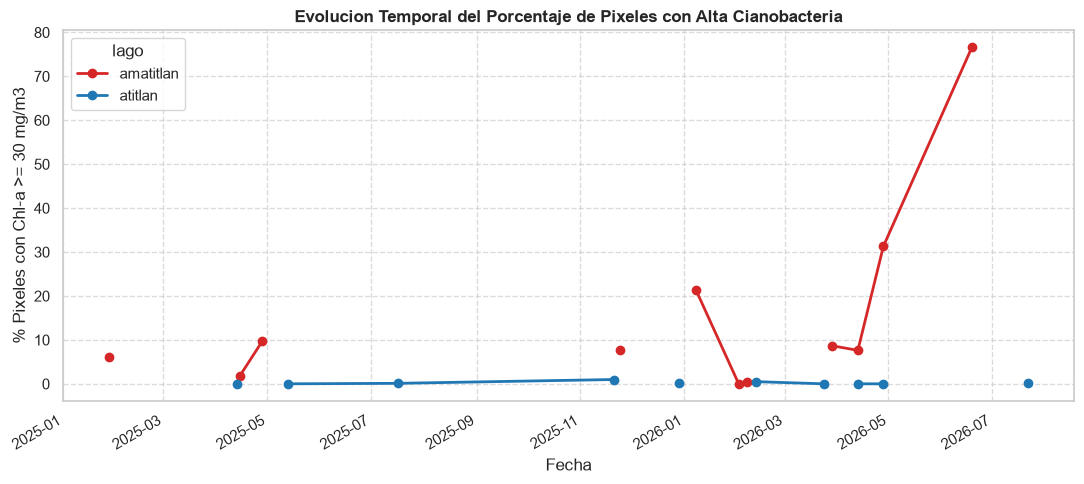
\includegraphics[width=0.9\textwidth]{evolucion_prevalencia.png}
    \caption{Evolución temporal del porcentaje de píxeles con alta cianobacteria, por lago.}
    \label{fig:evolucion_prevalencia}
\end{figure}

\subsection{Desbalance de clases}

La razón entre clase minoritaria y mayoritaria es de aproximadamente \textbf{1:50} (3{,}256{,}123 observaciones negativas contra 65{,}204 positivas). Esto tiene varias consecuencias directas para el modelado:

\begin{enumerate}
    \item \textbf{El Accuracy no sirve como métrica principal.} Predecir siempre la clase 0 acertaría el 98.04\,\% de las veces sin detectar una sola floración.
    \item \textbf{Las funciones de pérdida ignoran, por defecto, a la clase minoritaria.} Con 1.96\,\% de positivos, sacrificarlos es el camino más barato para minimizar el error total. Por eso se usó \texttt{class\_weight='balanced'} en Regresión Logística y Random Forest, y \texttt{scale\_pos\_weight} en XGBoost.
    \item \textbf{Se prioriza Recall, Precision, F1 y ROC-AUC} sobre el Accuracy en toda la evaluación posterior.
    \item \textbf{El desbalance no es igual en los dos lagos:} 0.21\,\% de positivos en Atitlán contra 15.56\,\% en Amatitlán, así que un modelo entrenado con ambos lagos aprende sobre todo del comportamiento de Amatitlán.
\end{enumerate}

\subsection{Variables que no pueden usarse como predictoras}

Dos variables participan directamente en la construcción de la respuesta y deben excluirse:

\begin{itemize}
    \item \textbf{\texttt{chla}.} La respuesta es \(y = \mathbb{1}(\text{Chl-}a \ge 30)\); usarla como predictora equivaldría a leer directamente el umbral.
    \item \textbf{\texttt{ndci}.} La clorofila se deriva del NDCI mediante \(\text{Chl-}a = 826.57\,\text{NDCI}^3 - 176.43\,\text{NDCI}^2 + 19\,\text{NDCI} + 4.071\). Al ser una función determinista de NDCI, incluirlo introduce la respuesta por la puerta de atrás.
\end{itemize}

En cambio, \texttt{B04} y \texttt{B05} sí se conservan: son los insumos crudos del NDCI, pero por separado no reconstruyen el umbral, y son justamente las bandas que aportan la señal física del borde rojo.

% ======================================================================
\section{Selección y construcción de variables predictoras}
\label{sec:predictores}
% ======================================================================

Se seleccionaron 17 predictores, resumidos en la Tabla~\ref{tab:predictores}.

\begin{table}[H]
\centering
\small
\caption{Variables predictoras utilizadas en los modelos.}
\label{tab:predictores}
\begin{tabular}{p{2.6cm}p{1.8cm}p{8.8cm}}
\toprule
Variable & Categoría & Qué representa / por qué puede ayudar \\
\midrule
B02 (490 nm) & Espectral & Reflectancia en el azul; el agua limpia dispersa mucho azul, la floración lo absorbe. \\
B03 (560 nm) & Espectral & Reflectancia en el verde; el reflejo característico del fitoplancton en superficie. \\
B04 (665 nm) & Espectral & Pico de absorción de la clorofila; crea el contraste con el infrarrojo cercano. \\
B05 (705 nm) & Espectral & Borde rojo; la banda más sensible a concentraciones altas de clorofila. \\
B07 (783 nm) & Espectral & Borde rojo lejano; responde a material particulado y floraciones en superficie. \\
B08 (842 nm) & Espectral & Infrarrojo cercano; el agua lo absorbe casi todo, así que biomasa flotante lo dispara. \\
B8A (865 nm) & Espectral & Infrarrojo cercano angosto; referencia para separar fondo de natas superficiales. \\
B11 (1610 nm) & Espectral & Infrarrojo de onda corta, muy absorbido por agua pura; se mueve con turbidez inorgánica. \\
B12 (2190 nm) & Espectral & Infrarrojo de onda corta lejano; ayuda a distinguir aerosoles, vapor y sedimento denso. \\
NDVI & Índice & Sube cuando hay biomasa flotante suficiente para comportarse como vegetación. \\
NDWI & Índice & Separa agua libre de agua cargada de materia orgánica. \\
distancia\_\newline orilla\_m & Espacial & Distancia a la orilla en metros; la costa recibe descargas de nutrientes (p. ej. río Villalobos). \\
x\_utm, y\_utm & Espacial & Coordenadas UTM 15N; capturan gradientes este-oeste y norte-sur dentro de cada lago. \\
mes & Temporal & Mes de la toma (1--12); recoge el ciclo anual de las floraciones. \\
estacion\_cod & Temporal & Época seca (nov--abr) o lluviosa (may--oct); la escorrentía lluviosa arrastra nutrientes. \\
indice\_turbidez\_\newline swir & Ingeniería & Razón B11/B08; distingue turbidez por sedimento de turbidez por algas. \\
\bottomrule
\end{tabular}
\end{table}

Es importante notar que, al ser coordenadas absolutas, \texttt{x\_utm} y \texttt{y\_utm} permiten al modelo memorizar la posición en lugar de aprender la señal espectral. La Sección~\ref{sec:validacion} valida con bloques espaciales, donde esas coordenadas dejan de servirle al modelo para ``hacer trampa'' dentro de un mismo lago, y la Sección~\ref{sec:interpretabilidad} cuantifica exactamente cuánto pesa ese atajo.

% ======================================================================
\section{Construcción de los modelos de Machine Learning}
\label{sec:modelos}
% ======================================================================

Se entrenaron tres modelos de clasificación:

\begin{enumerate}
    \item \textbf{Regresión Logística:} imputación por mediana, \texttt{StandardScaler}, regularización L2 con \(C=1.0\) y \texttt{class\_weight='balanced'}.
    \item \textbf{Random Forest:} \texttt{n\_estimators=80}, \texttt{max\_depth=12}, \texttt{class\_weight='balanced'}, \texttt{max\_samples=0.20}.
    \item \textbf{XGBoost:} \texttt{tree\_method='hist'}, \texttt{learning\_rate=0.1}, \texttt{max\_depth=6}, con \texttt{scale\_pos\_weight} igual a la razón de negativos sobre positivos en el conjunto de entrenamiento.
\end{enumerate}

\textbf{Sobre el tamaño de la muestra.} Entrenar Random Forest sobre los 3.3 millones de píxeles, cinco veces por cada fold de validación espacial, no era viable en el equipo de cómputo disponible. Se trabajó con una muestra de \textbf{250{,}000 píxeles}, estratificada por lago y por clase, que conserva tanto la proporción de positivos como el peso relativo de cada lago. Todos los ejercicios de modelado (4 a 9) usan esta misma muestra.

\textbf{División de datos.} 70\,\% entrenamiento y 30\,\% prueba, estratificado por clase (\texttt{stratify=y}, \texttt{random\_state=42}): 174{,}999 observaciones de entrenamiento (3{,}433 positivas) y 75{,}000 de prueba (1{,}472 positivas). Los tres modelos se evalúan sobre exactamente el mismo conjunto de prueba.

\textbf{Por qué esos hiperparámetros.}

\emph{Regresión Logística.} \texttt{StandardScaler} porque las bandas y los índices están en escalas distintas, y sin normalizar las variables de valores grandes dominarían los coeficientes. \texttt{class\_weight='balanced'} es indispensable con solo 1.96\,\% de positivos. \(C=1.0\) regulariza la fuerte colinealidad entre bandas mostrada en la Figura~\ref{fig:correlacion}.

\emph{Random Forest.} Se probó \texttt{n\_estimators} en 50, 80 y 150: de 80 en adelante las métricas ya no cambiaban. \texttt{max\_depth=12} evita que el modelo memorice ruido radiométrico. \texttt{min\_samples\_leaf=5} evita hojas de un solo píxel. \texttt{max\_samples=0.20} mantiene la diversidad del ensamble y reduce el costo de entrenamiento.

\emph{XGBoost.} \texttt{scale\_pos\_weight} compensa el desbalance directamente en el gradiente. \texttt{learning\_rate=0.1} con \texttt{n\_estimators=100}: con tasas más altas el modelo se volvía inestable entre folds. \texttt{subsample} y \texttt{colsample\_bytree} de 0.8 evitan que los árboles dependan siempre de las mismas bandas. \texttt{tree\_method='hist'} hace viable entrenar con cientos de miles de filas en tiempos razonables.

% ======================================================================
\section{Evaluación de los modelos}
\label{sec:evaluacion}
% ======================================================================

\subsection{Métricas sobre el conjunto de prueba}

\begin{table}[H]
\centering
\caption{Rendimiento de los tres modelos sobre el conjunto de prueba fijo (30\,\%), división aleatoria 70/30.}
\label{tab:metricas_test}
\begin{tabular}{lrrrrr}
\toprule
Modelo & Accuracy & Precision & Recall & F1-Score & ROC-AUC \\
\midrule
Regresión Logística & 0.9937 & 0.7582 & 0.9993 & 0.8623 & 0.9998 \\
Random Forest        & 0.9891 & 0.6459 & 0.9851 & 0.7802 & 0.9991 \\
XGBoost               & 0.9951 & 0.8092 & 0.9823 & \textbf{0.8874} & 0.9997 \\
\bottomrule
\end{tabular}
\end{table}

\begin{figure}[H]
    \centering
    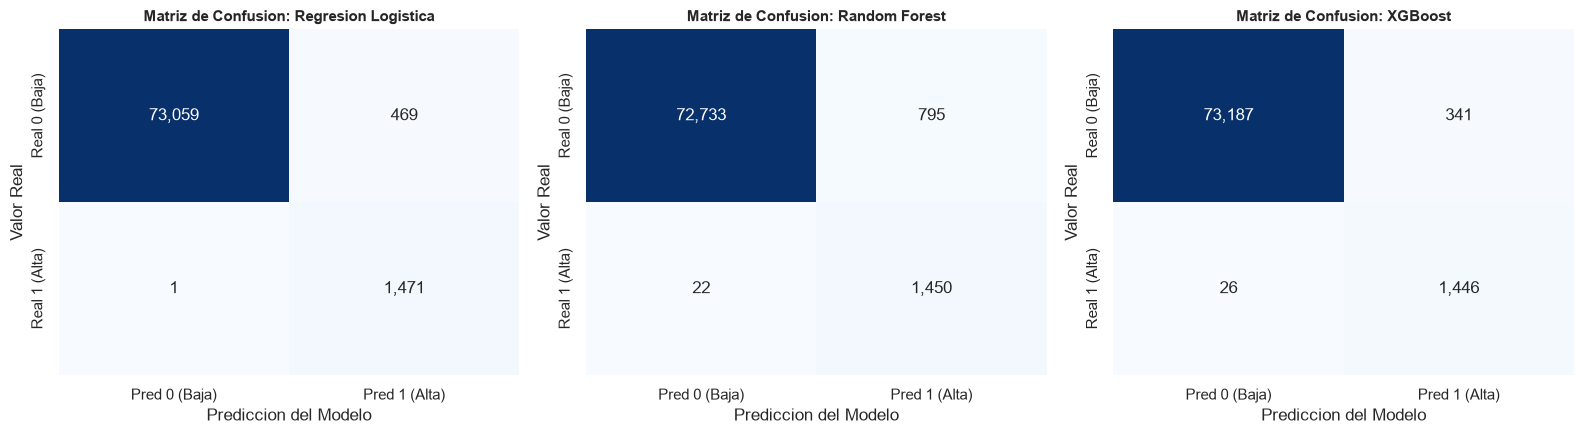
\includegraphics[width=\textwidth]{matrices_confusion.png}
    \caption{Matrices de confusión de los tres modelos sobre el conjunto de prueba.}
    \label{fig:matrices_confusion}
\end{figure}

\begin{figure}[H]
    \centering
    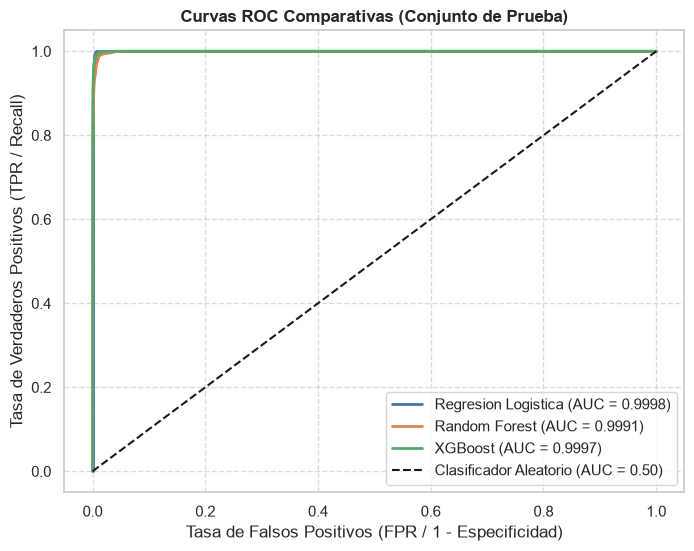
\includegraphics[width=0.7\textwidth]{curvas_roc.png}
    \caption{Curvas ROC comparativas de los tres modelos sobre el conjunto de prueba.}
    \label{fig:curvas_roc}
\end{figure}

\subsection{Comparación de los tres modelos}

\textbf{XGBoost es el mejor modelo}: el F1 más alto (0.8874) con la mejor precisión del grupo (0.8092) y un Recall de 0.9823. La \textbf{Regresión Logística} logra el Recall más alto (0.9993) pero con precisión de solo 0.7582, porque para no perder positivos abre demasiado la frontera de decisión. \textbf{Random Forest} queda último en precisión (0.6459): la combinación de \texttt{class\_weight='balanced'} con \texttt{max\_samples=0.20} lo vuelve muy agresivo con la clase minoritaria y marca bastante más área de la que corresponde.

Los tres modelos superan 0.999 de ROC-AUC, es decir, ordenan igual de bien a los píxeles por nivel de riesgo. La diferencia entre ellos está en dónde cae el umbral de decisión de 0.5, no en su capacidad de discriminación subyacente.

\subsection{Qué error importa más desde el punto de vista ambiental}

\textbf{Falso negativo (no detectar una floración real).} La gente sigue usando el agua mientras hay cianotoxinas presentes, no se activan los planes de contingencia, y el daño a la salud pública ya está hecho para cuando la floración se detecta por otra vía. Es el error grave.

\textbf{Falso positivo (marcar floración donde no la hay).} Se envía a alguien a muestrear de más, o se restringe el uso del agua unos días sin necesidad real. Cuesta tiempo y dinero y molesta al turismo, pero es un error reversible.

Como el costo de ambos errores es tan disparejo, se prioriza el \textbf{Recall} como métrica de decisión, usando F1 y ROC-AUC como control para no premiar a un modelo que alcance sensibilidad alta simplemente marcando todo el lago como positivo -- que es justamente el problema de Random Forest en este caso.

% ======================================================================
\section{Validación espacial y temporal}
\label{sec:validacion}
% ======================================================================

\subsection{Por qué una cuadrícula de 1 km}

Dos píxeles vecinos, separados por apenas 20 metros, tienen casi la misma reflectancia. Si se reparten al azar entre entrenamiento y prueba, el modelo puede acertar por vecindad en lugar de por haber aprendido un patrón real, y las métricas de la Sección~\ref{sec:evaluacion} salen infladas. Para medir ese efecto se dividió cada lago en bloques de 1000 por 1000 metros sobre EPSG:32615 (trabaja en metros y cubre ambos lagos).

Antes de fijar ese tamaño se comparó contra 500 m y 2 km (Tabla~\ref{tab:tamano_bloques}):

\begin{table}[H]
\centering
\small
\caption{Comparación de tamaños de cuadrícula espacial.}
\label{tab:tamano_bloques}
\begin{tabular}{lrrr}
\toprule
 & 500 m & 1000 m & 2000 m \\
\midrule
Bloques totales & 668 & 198 & 64 \\
Bloques en Atitlán & 571 & 165 & 51 \\
Bloques en Amatitlán & 97 & 33 & 13 \\
Mediana de píxeles por bloque & 6{,}245 & 21{,}814 & 44{,}371 \\
Bloques con menos de 100 píxeles & 16 & 4 & 2 \\
Bloques con algún positivo & 557 & 189 & 63 \\
Bloques de Amatitlán por fold (de 5) & 19.4 & 6.6 & 2.6 \\
\bottomrule
\end{tabular}
\end{table}

Con 500 m quedan 668 bloques, pero solo 557 contienen algún positivo y 16 caen bajo 100 observaciones: demasiados grupos degenerados sin clase positiva. Con 2 km solo hay 64 bloques y Amatitlán se queda con 13, es decir 2.6 por fold: muy pocos para que la validación de ese lago signifique algo. Con \textbf{1 km}, 189 de los 198 bloques tienen al menos un positivo y solo 4 caen bajo 100 observaciones (0.004\,\% de los datos). El factor decisivo es el tamaño de Amatitlán: con 13.8 km\(^2\) de espejo de agua, cualquier cuadrícula más gruesa lo deja sin bloques suficientes para repartir entre 5 folds.

\begin{figure}[H]
    \centering
    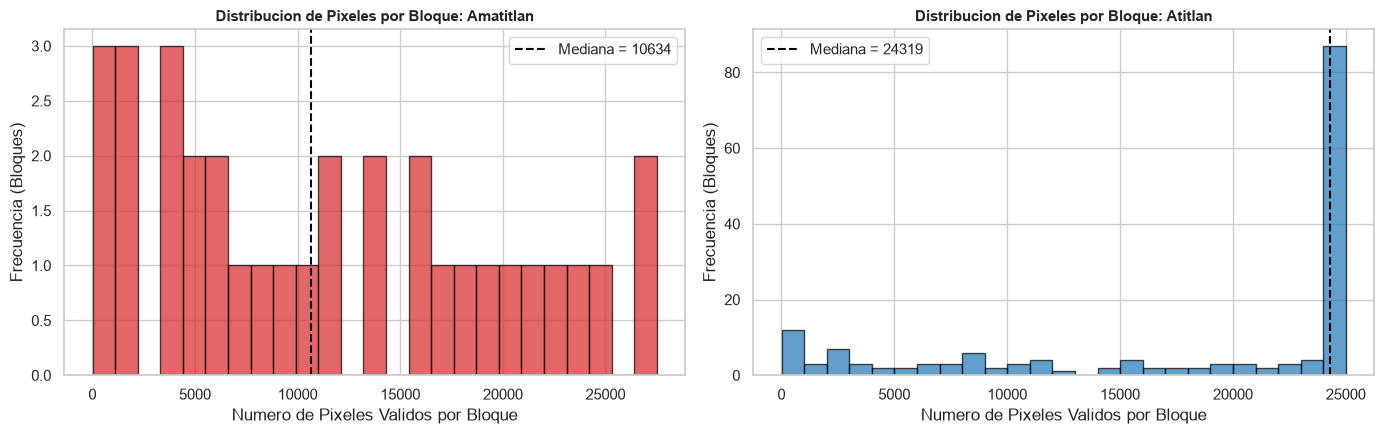
\includegraphics[width=0.85\textwidth]{histograma_bloques.png}
    \caption{Distribución del número de píxeles válidos por bloque de 1 km, por lago.}
    \label{fig:histograma_bloques}
\end{figure}

\begin{figure}[H]
    \centering
    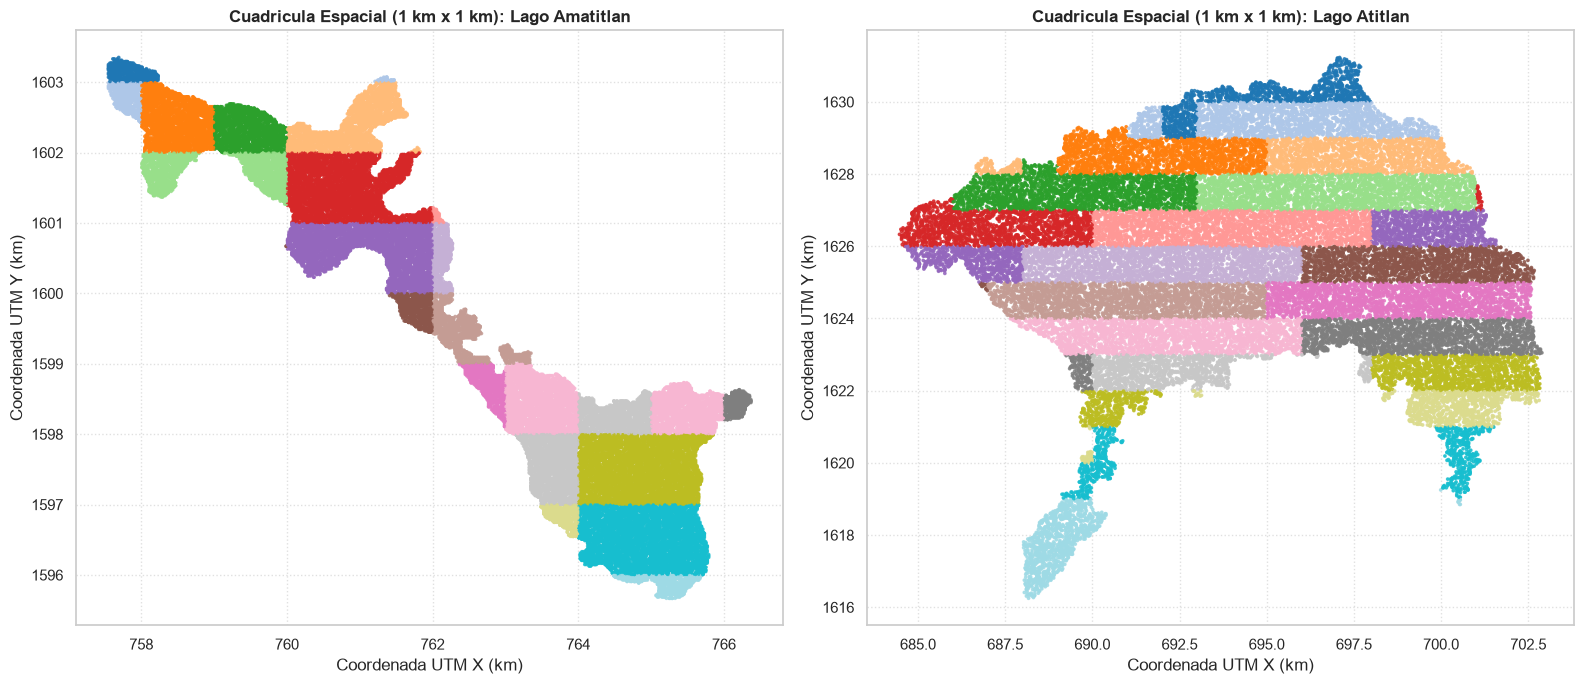
\includegraphics[width=0.95\textwidth]{cuadricula_espacial.png}
    \caption{Cuadrícula espacial de 1 km $\times$ 1 km asignada a cada píxel, Amatitlán (izquierda) y Atitlán (derecha). Cada color representa un bloque distinto.}
    \label{fig:cuadricula_espacial}
\end{figure}

\subsection{Validación cruzada espacial (GroupKFold)}

Se usó \texttt{GroupKFold(n\_splits=5)} agrupando por el identificador de bloque. Todos los píxeles de un mismo bloque de 1 km caen juntos en entrenamiento o en validación, nunca repartidos entre ambos; como el bloque depende solo de la posición, esto también agrupa las distintas fechas de una misma zona, así que el modelo tampoco puede reconocer un lugar por haberlo visto en otra fecha.

\begin{table}[H]
\centering
\caption{Aleatoria (70/30) contra espacial (GroupKFold, bloques de 1 km): F1-Score.}
\label{tab:aleatoria_espacial}
\begin{tabular}{lrr}
\toprule
Modelo & F1 aleatorio & F1 espacial \\
\midrule
Regresión Logística & 0.8623 & 0.8637 \\
Random Forest & 0.7802 & 0.7727 \\
XGBoost & 0.8874 & 0.8850 \\
\bottomrule
\end{tabular}
\end{table}

\begin{figure}[H]
    \centering
    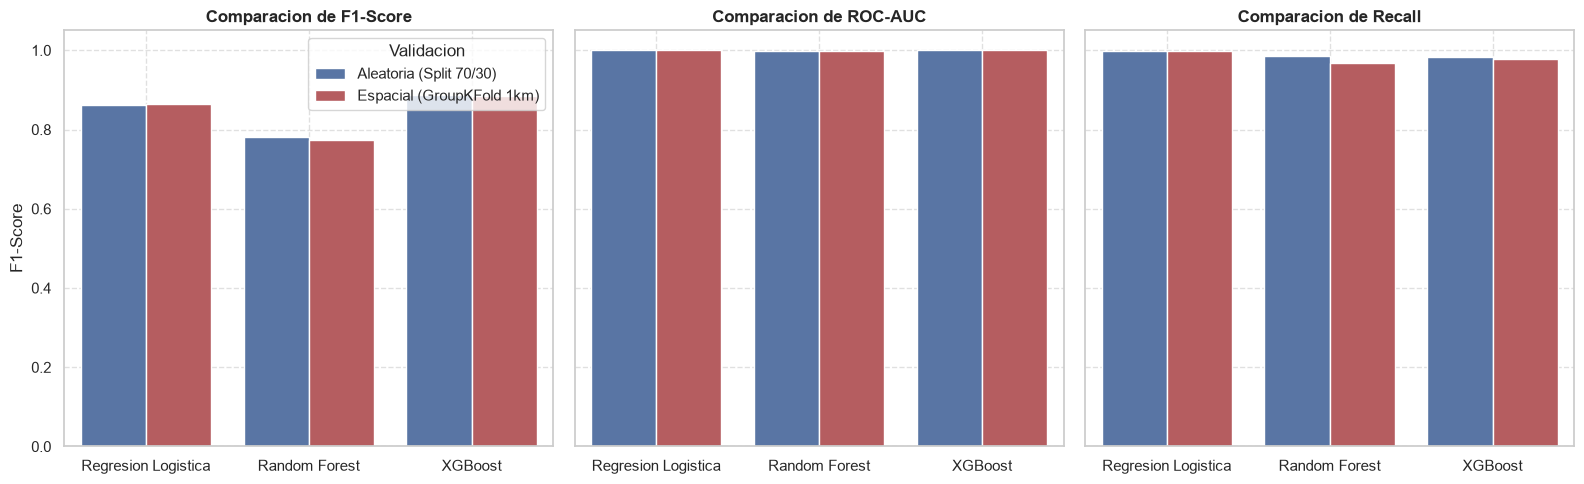
\includegraphics[width=\textwidth]{comparacion_aleatoria_espacial.png}
    \caption{F1-Score, ROC-AUC y Recall bajo validación aleatoria contra validación espacial.}
    \label{fig:comparacion_aleatoria_espacial}
\end{figure}

\textbf{La caída es mínima.} Ningún modelo pierde un punto completo de F1; Random Forest baja algo en Recall (de 0.9851 a 0.9671) y los otros dos se mantienen prácticamente igual.

Por la primera ley de Tobler (``las cosas cercanas se parecen más entre sí''), se esperaba una caída: en una división aleatoria por píxeles, un píxel de prueba puede estar a 20 metros de uno de entrenamiento, y el modelo acierta por vecindad. Agrupar por bloques de 1 km cierra esa ruta. Que la caída no se materialice se explica en la Sección~\ref{sec:interpretabilidad}: la cuadrícula separa vecindarios \emph{dentro} de un lago, pero los dos lagos siguen presentes en entrenamiento y validación en todos los folds, y el modelo se apoya en \texttt{y\_utm} como identificador de lago -- una pista que sobrevive intacta a la partición por bloques. Sin embargo, el mismo análisis de interpretabilidad muestra que el modelo no necesitaba esa pista: reentrenado sin coordenadas, el F1 no baja (de hecho sube ligeramente). Las dos cosas son ciertas a la vez: el modelo tomó un atajo posicional, y aun sin él habría funcionado igual de bien dentro de un lago.

\subsection{Validación temporal}

La validación por bloques responde qué tan bien predice el modelo sobre una zona que no vio. Falta la otra mitad de la pregunta, la que más importa para un sistema de alerta real: qué tan bien predice sobre una \textbf{fecha} que no vio. En operación, el modelo se entrena con las imágenes que existen hasta hoy y se aplica a la imagen que baja mañana; nunca tiene ejemplos del futuro.

Se usó \texttt{TimeSeriesSplit} con 4 folds sobre las 19 fechas ordenadas cronológicamente, con ventana expansiva: cada fold entrena con todas las fechas anteriores a un corte y valida sobre las tres siguientes, de modo que el entrenamiento siempre precede a la validación en el tiempo.

\begin{table}[H]
\centering
\caption{Las tres estrategias de validación, lado a lado (F1-Score).}
\label{tab:tres_estrategias}
\begin{tabular}{lrrr}
\toprule
Modelo & Aleatoria (70/30) & Espacial (bloques 1 km) & Temporal (por fecha) \\
\midrule
Regresión Logística & 0.8623 & 0.8637 & 0.7637 \\
Random Forest        & 0.7802 & 0.7727 & 0.6265 \\
XGBoost               & 0.8874 & 0.8850 & 0.7031 \\
\bottomrule
\end{tabular}
\end{table}

\begin{figure}[H]
    \centering
    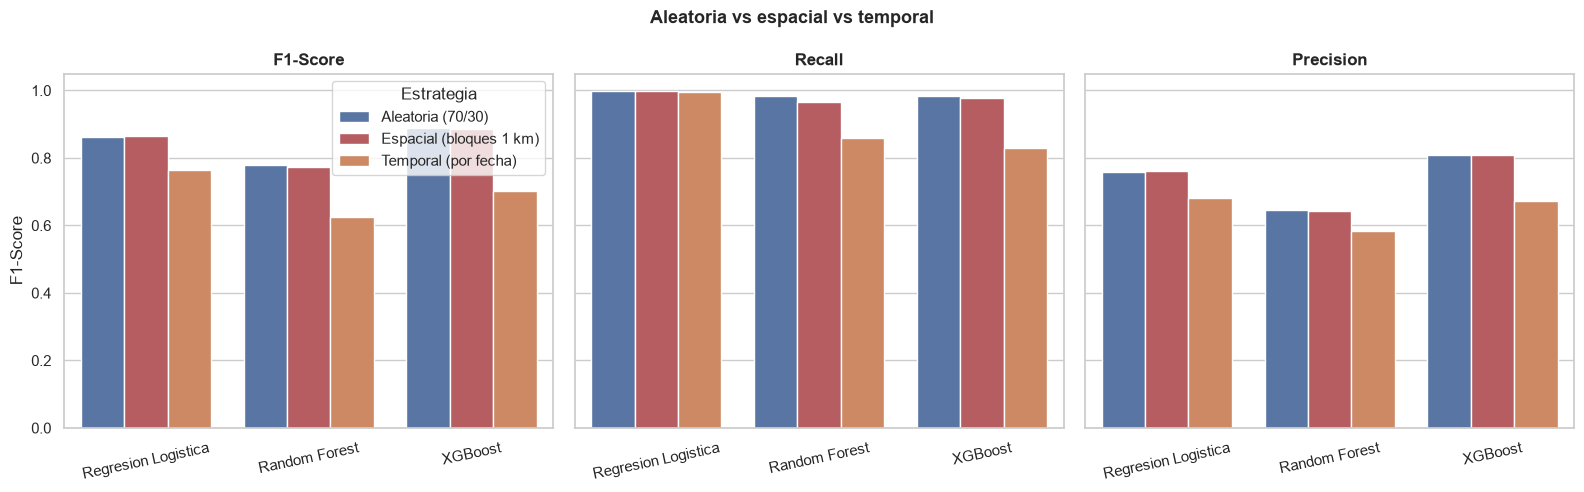
\includegraphics[width=\textwidth]{comparacion_tres_estrategias.png}
    \caption{F1-Score, Recall y Precision bajo las tres estrategias de validación: aleatoria, espacial y temporal.}
    \label{fig:comparacion_tres_estrategias}
\end{figure}

\textbf{Aquí sí hay caída, y es la mayor de todo el laboratorio.} Separar el espacio no costó nada; separar el tiempo cuesta entre 0.10 y 0.18 puntos de F1, y el modelo más castigado es justamente XGBoost, el mejor bajo las otras dos validaciones (F1 baja de 0.8874 a 0.7031). Lo que limita a este modelo no es la geografía, sino el calendario.

El desempeño de cada fold sigue de cerca la prevalencia de su ventana temporal: el fold que valida sobre febrero de 2026 (0.35\,\% de positivos) se desploma a F1 = 0.388 para XGBoost, mientras que el fold que incluye el evento de Amatitlán 2026-06-19 llega a F1 = 0.892. Agrupar por bloques quita el vecindario inmediato pero conserva los dos lagos y todas las fechas; agrupar por fecha quita, en cambio, variables que el modelo sí usaba (\texttt{mes} y \texttt{estacion\_cod}, ver Sección~\ref{sec:interpretabilidad}) y suma diferencias de corrección atmosférica, ángulo solar y satélite entre escenas. Para un sistema que se entrena con el histórico y predice la imagen de mañana, la referencia honesta es \textbf{F1 = 0.7031}, no el 0.8874 de la división aleatoria.

% ======================================================================
\section{Generalización entre lagos}
\label{sec:generalizacion}
% ======================================================================

Hasta este punto los modelos siempre vieron ambos lagos durante el entrenamiento. Aquí se separan por completo: el \textbf{Experimento A} entrena solo con Atitlán y evalúa sobre Amatitlán; el \textbf{Experimento B} hace lo contrario. Los dos lagos son casi opuestos: Atitlán es profundo, oligotrófico (0.21\,\% de positivos); Amatitlán es somero, hipereutrófico (15.56\,\% de positivos).

\begin{table}[H]
\centering
\caption{XGBoost: mismo lago contra transferencia entre lagos.}
\label{tab:generalizacion}
\begin{tabular}{lrrrr}
\toprule
Escenario & Precision & Recall & F1-Score & ROC-AUC \\
\midrule
Entrena y evalúa en Atitlán (70/30) & 0.5020 & 0.9137 & 0.6480 & 0.9988 \\
Entrena y evalúa en Amatitlán (70/30) & 0.9318 & 0.9745 & 0.9527 & 0.9987 \\
Entrena Atitlán, evalúa Amatitlán & 0.8438 & 0.1909 & 0.3114 & 0.8056 \\
Entrena Amatitlán, evalúa Atitlán & 0.7778 & 0.3319 & 0.4653 & 0.9036 \\
\bottomrule
\end{tabular}
\end{table}

\begin{figure}[H]
    \centering
    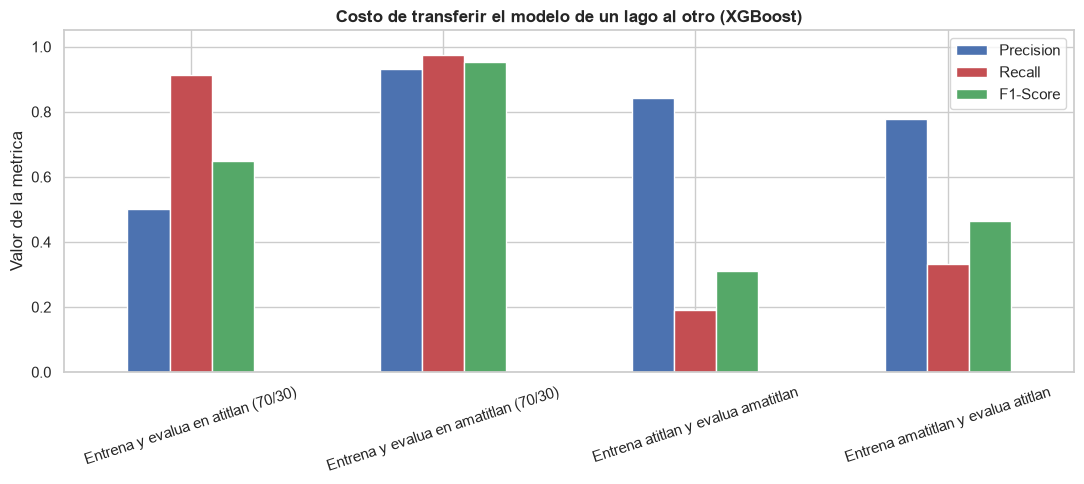
\includegraphics[width=0.75\textwidth]{costo_transferencia_lagos.png}
    \caption{Costo de transferir el modelo XGBoost de un lago al otro, comparado contra entrenar y evaluar en el mismo lago.}
    \label{fig:costo_transferencia}
\end{figure}

En ambos cruces el Recall cae de más del 91\,\% (dentro de un lago) a entre 19\,\% y 33\,\% (entre lagos). La precisión aguanta razonablemente bien, así que cuando el modelo transferido marca algo suele acertar, pero se le escapa la mayoría de los eventos reales -- el peor perfil posible para un sistema de alerta temprana.

\textbf{¿Generaliza un modelo de un lago al otro? Depende del modelo.} La Regresión Logística entrenada solo con Atitlán detecta las floraciones de Amatitlán con F1 = 0.9510, habiendo visto apenas 464 píxeles positivos durante el entrenamiento. La razón es la extrapolación: Amatitlán presenta reflectancias de borde rojo por encima de todo lo observado en Atitlán, y un modelo basado en árboles devuelve una constante más allá de su último corte de decisión, mientras que un modelo lineal prolonga la tendencia; como ``más borde rojo implica más clorofila'' es aproximadamente monótono, esa prolongación acierta. En la dirección contraria falla todo (F1 máximo de 0.4653 con XGBoost), y la causa aquí es la prevalencia: un umbral calibrado donde 1 de cada 6 píxeles está en floración es inservible donde la proporción es 1 de cada 480.

Un control adicional descarta que las coordenadas expliquen esta falla: sin \texttt{x\_utm} ni \texttt{y\_utm}, XGBoost pasa de F1 = 0.3114 a 0.3175 en un sentido y de 0.4653 a 0.4635 en el otro -- prácticamente sin cambio. Lo que falla es el ajuste a las distribuciones espectrales y a la prevalencia de cada lago, no las coordenadas fuera de rango.

Cuatro diferencias entre los lagos explican esta falta de transferencia: (1) el \textbf{régimen trófico} opuesto (0.21\,\% contra 15.56\,\% de prevalencia, así que cualquier umbral queda mal calibrado en el otro lago); (2) el \textbf{fondo espectral} distinto (Atitlán es una caldera profunda de agua clara, Amatitlán es somero y turbio por el sedimento del río Villalobos, así que el mismo valor de reflectancia no significa lo mismo en ambos); (3) el \textbf{rango dinámico} (las concentraciones extremas de Amatitlán simplemente no ocurren en Atitlán, y ahí los modelos de árboles no tienen cómo extrapolar); y (4) la \textbf{morfometría} (casi todo Amatitlán está cerca de la orilla, mientras Atitlán tiene grandes extensiones de agua abierta, así que \texttt{distancia\_orilla\_m} no es comparable entre ambos). La conclusión práctica es que no conviene trasladar un modelo entrenado en un lago a otro lago sin datos etiquetados de ese segundo lago; si hubiera que intentarlo de todas formas, la evidencia aquí favorece el modelo lineal sobre los basados en árboles, justo lo contrario de lo que sugieren las métricas dentro de un solo lago.

% ======================================================================
\section{Interpretación y explicabilidad del modelo}
\label{sec:interpretabilidad}
% ======================================================================

\subsection{Importancia global de las variables}

Se tomó el mejor modelo, XGBoost entrenado sobre la división 70/30, y se examinó en qué variables se apoya mediante la importancia por ganancia (cuánto mejora la función de pérdida cada vez que un árbol corta por esa variable).

\begin{figure}[H]
    \centering
    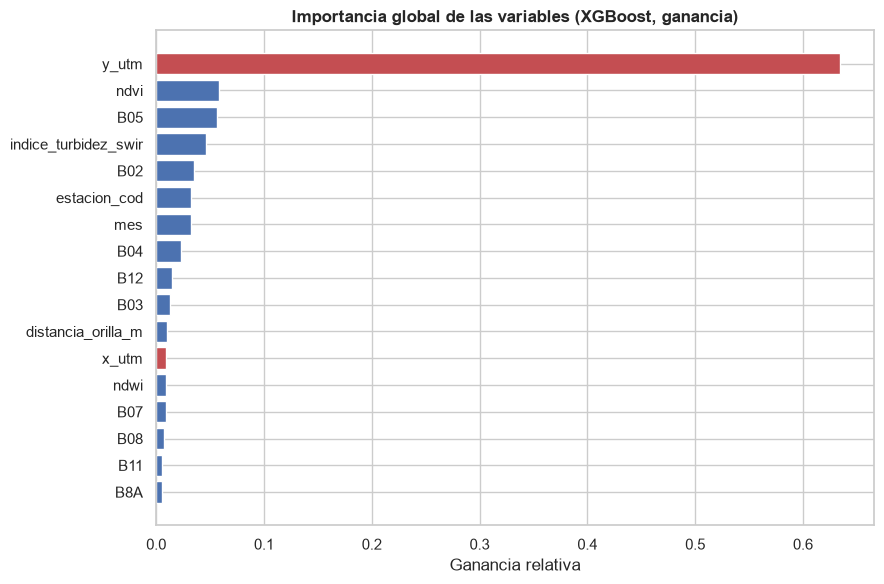
\includegraphics[width=0.7\textwidth]{importancia_variables.png}
    \caption{Importancia global de las variables en XGBoost (ganancia relativa). Las coordenadas se resaltan en rojo.}
    \label{fig:importancia_variables}
\end{figure}

Por ganancia, \texttt{y\_utm} domina con el 63.4\,\% del total, más de tres veces lo que suman las nueve bandas espectrales juntas (16.9\,\%).

\subsection{SHAP}

La importancia por ganancia indica cuánto usa el modelo cada variable, pero no en qué dirección empuja la predicción. SHAP (SHapley Additive exPlanations) reparte cada predicción individual entre las variables que la empujaron hacia arriba o hacia abajo. Los valores se calcularon sobre una muestra sobrerrepresentando la clase positiva (1{,}500 píxeles con floración y 6{,}000 sin ella, de 7{,}472 en total), porque con la proporción natural de clases casi todos los puntos serían negativos y el gráfico no mostraría nada útil.

\begin{figure}[H]
    \centering
    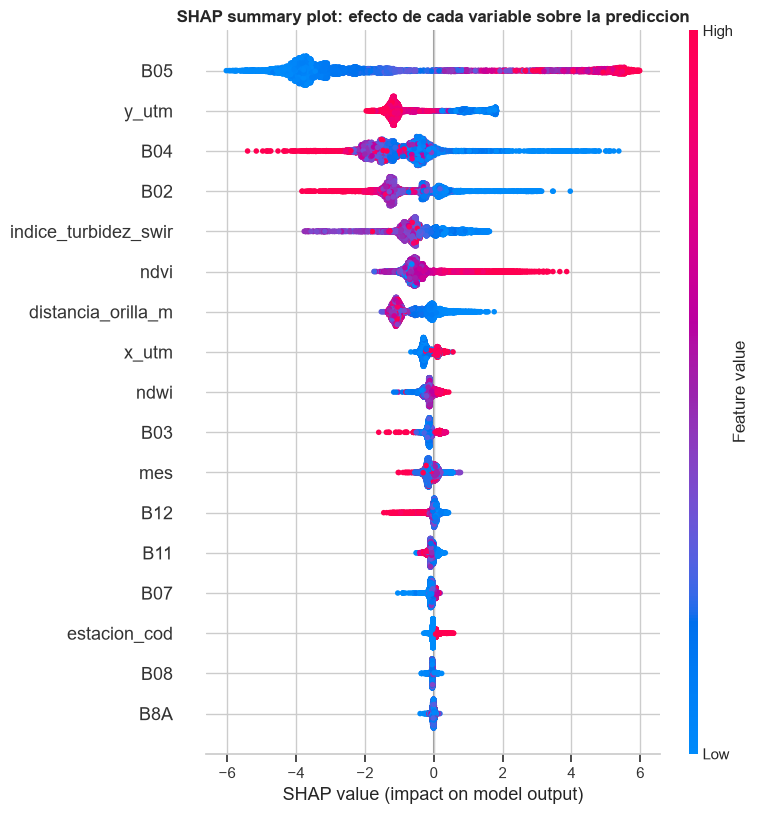
\includegraphics[width=0.6\textwidth]{shap_summary.png}
    \caption{SHAP summary plot: efecto de cada variable sobre la predicción de alta cianobacteria.}
    \label{fig:shap_summary}
\end{figure}

\begin{figure}[H]
    \centering
    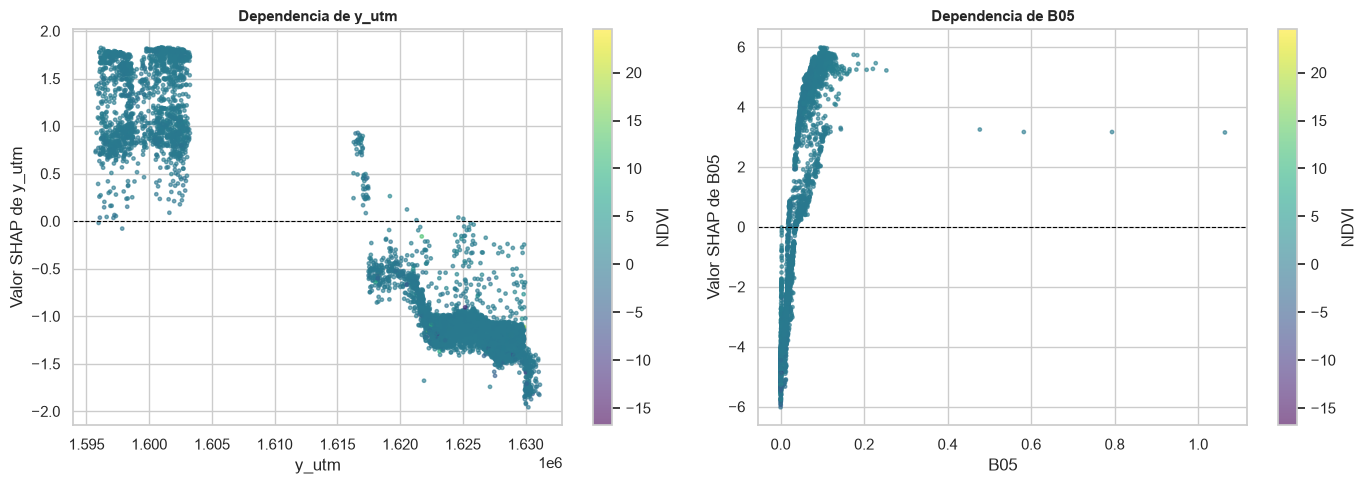
\includegraphics[width=0.95\textwidth]{shap_dependencia.png}
    \caption{Gráficos de dependencia SHAP para \texttt{y\_utm} (izquierda) y \texttt{B05} (derecha), coloreados por NDVI.}
    \label{fig:shap_dependencia}
\end{figure}

Las dos medidas de importancia \textbf{no ordenan igual} las variables (correlación de Spearman de 0.740 entre ambos rankings). Por SHAP medio, \texttt{B05} queda primera y \texttt{y\_utm} segunda con menos de la mitad de su peso relativo. No es una contradicción: la ganancia premia los cortes cercanos a la raíz del árbol, y \texttt{y\_utm} hace exactamente eso -- un corte cercano a la raíz separa los dos lagos y elimina de golpe buena parte de la incertidumbre, porque las prevalencias de base son tan distintas (0.21\,\% contra 15.56\,\%). Una vez hecha esa separación, quien decide píxel por píxel es \texttt{B05}, que es lo que mide SHAP. En una frase: \textbf{\texttt{y\_utm} sirve para ubicarse, y \texttt{B05} para decidir}.

\textbf{El atajo posicional no era necesario.} Al remover \texttt{x\_utm} y \texttt{y\_utm} del modelo, el F1 pasa de 0.8874 a 0.8892 y el Recall de 0.9823 a 0.9891 -- una mejora marginal, no una caída. Esto explica retrospectivamente por qué la validación espacial de la Sección~\ref{sec:validacion} resultó poco exigente: nunca puso a prueba la pista de ubicación que el modelo usaba, porque los bloques de 1 km no separan lagos. En retrospectiva, las coordenadas no debieron incluirse en un modelo entrenado con dos lagos a la vez.

\begin{table}[H]
\centering
\small
\caption{Sentido físico de las variables con mayor peso SHAP.}
\label{tab:shap_direccion}
\begin{tabular}{p{2.6cm}p{3.2cm}p{7cm}}
\toprule
Variable & Valores altos empujan hacia & Por qué \\
\midrule
B05 (borde rojo) & Floración & Es donde la clorofila deja su firma espectral. \\
B04 (rojo) & Sin floración & Pico de absorción: mucha reflectancia implica poca clorofila. \\
B02 (azul) & Sin floración & El agua limpia dispersa azul; los pigmentos lo absorben. \\
NDVI & Floración & Sube cuando la biomasa flotante responde como vegetación. \\
indice\_turbidez\_\newline swir & Sin floración & Separa turbidez mineral de la causada por algas. \\
distancia\_\newline orilla\_m & Sin floración & Los nutrientes entran por la costa. \\
y\_utm & Sin floración & Atitlán está al norte y es el lago de prevalencia baja. \\
\bottomrule
\end{tabular}
\end{table}

Que seis de estas siete variables coincidan con lo esperado desde la limnología es evidencia de que el modelo no está explotando artefactos de la imagen. La única variable sin un mecanismo físico directo es \texttt{y\_utm}, justamente la que la Sección~\ref{sec:generalizacion} muestra que no ayuda a generalizar entre lagos. El calendario (\texttt{mes}, \texttt{estacion\_cod}) pesa bastante por ganancia pero casi nada por SHAP: sirve para cortes gruesos, no para afinar predicciones individuales, y es justamente lo que penaliza a la validación temporal.

% ======================================================================
\section{Generación de mapas predictivos}
\label{sec:mapas}
% ======================================================================

Se aplicó XGBoost píxel por píxel sobre una fecha completa de cada lago (no la muestra de 250{,}000, sino todos los píxeles válidos de esa fecha) y se reconstruyeron las predicciones en su posición original. Se eligieron \textbf{Amatitlán 2026-06-19} (la floración más extensa de toda la serie, 76.6\,\% del lago sobre el umbral) y \textbf{Atitlán 2025-11-21} (la fecha con más área en floración de ese lago, aunque apenas 1\,\% de la superficie).

\begin{figure}[H]
    \centering
    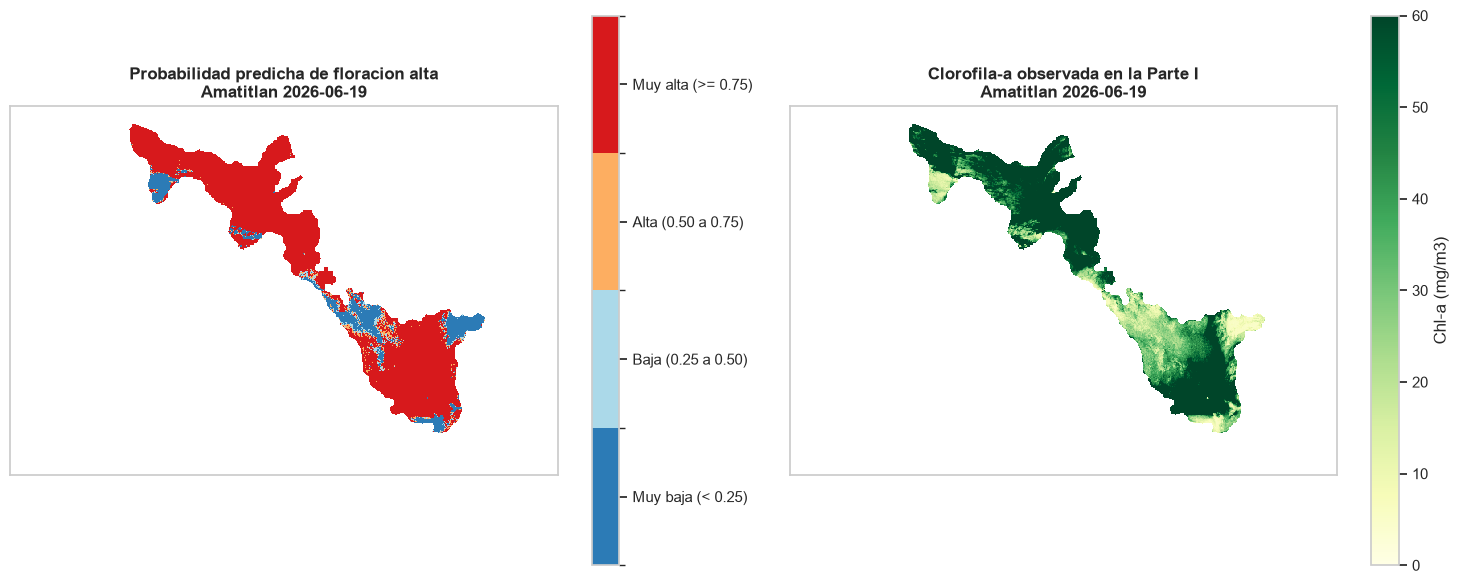
\includegraphics[width=0.95\textwidth]{mapa_predictivo_amatitlan.png}
    \caption{Amatitlán, 2026-06-19: probabilidad predicha de alta cianobacteria (izquierda) contra clorofila-\(a\) observada en la Parte I (derecha).}
    \label{fig:mapa_amatitlan}
\end{figure}

\begin{figure}[H]
    \centering
    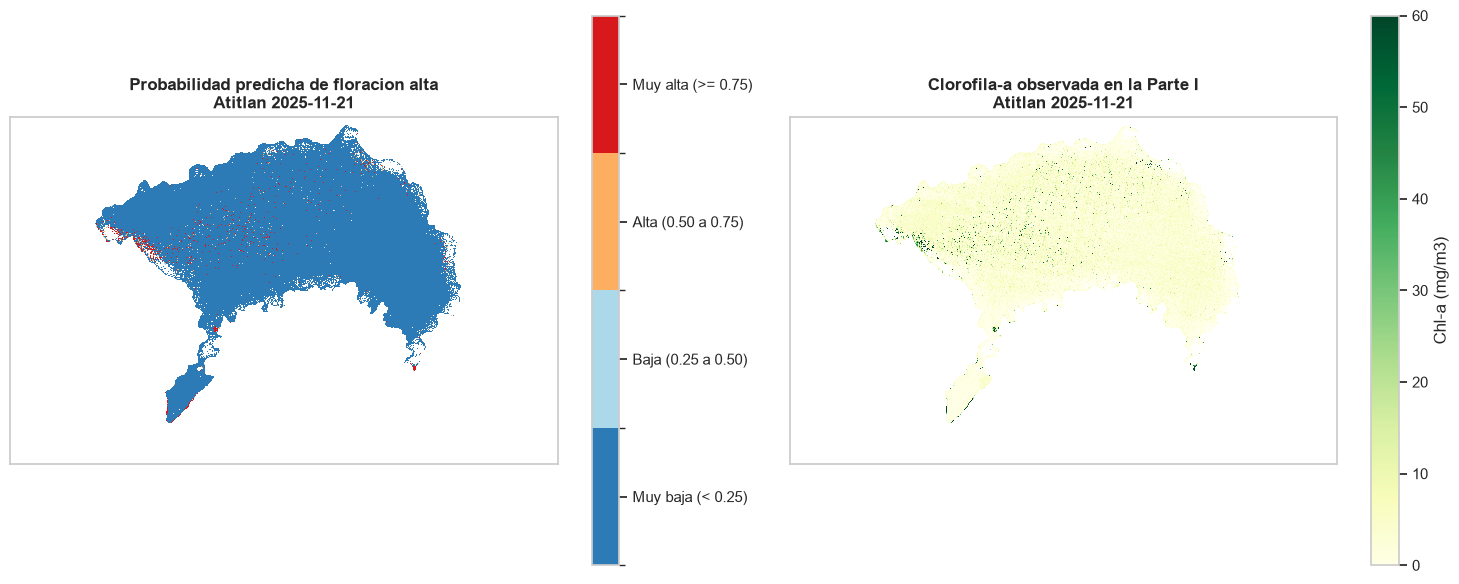
\includegraphics[width=0.95\textwidth]{mapa_predictivo_atitlan.png}
    \caption{Atitlán, 2025-11-21: probabilidad predicha de alta cianobacteria (izquierda) contra clorofila-\(a\) observada en la Parte I (derecha).}
    \label{fig:mapa_atitlan}
\end{figure}

\begin{figure}[H]
    \centering
    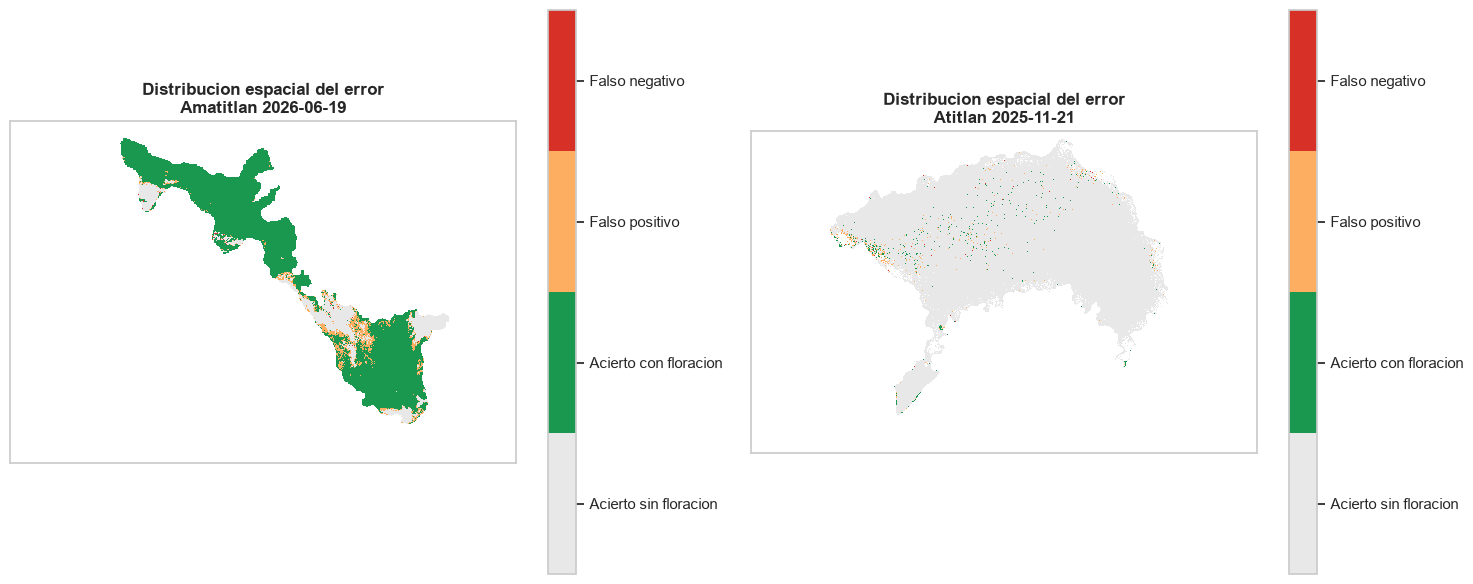
\includegraphics[width=0.95\textwidth]{mapa_errores.png}
    \caption{Distribución espacial del error de clasificación (aciertos, falsos positivos y falsos negativos) para las mismas dos fechas.}
    \label{fig:mapa_errores}
\end{figure}

\begin{table}[H]
\centering
\caption{Resumen numérico de los dos mapas predictivos.}
\label{tab:resumen_mapas}
\begin{tabular}{lrr}
\toprule
 & Amatitlán 2026-06-19 & Atitlán 2025-11-21 \\
\midrule
Recall & 0.9981 & 0.9196 \\
Precision & 0.9154 & 0.5204 \\
F1-Score & 0.9550 & 0.6646 \\
Falsos positivos & 2{,}432 & 2{,}426 \\
Falsos negativos & 49 & 230 \\
\bottomrule
\end{tabular}
\end{table}

\textbf{El mapa reproduce la forma real de la floración.} La probabilidad predicha y la clorofila-\(a\) de la Parte I coinciden en extensión y ubicación de los parches. En Amatitlán 2026-06-19 el lago aparece cubierto casi por completo (27{,}867 de 34{,}436 píxeles en probabilidad muy alta); en Atitlán 2025-11-21 el centro del lago queda en probabilidad muy baja y el riesgo se concentra en parches costeros.

El \textbf{número absoluto} de falsos positivos es casi idéntico en ambos lagos (alrededor de 2{,}430), pero contra bases muy distintas: en Amatitlán hay 26{,}380 positivos reales y esa cantidad de errores es ruido menor; en Atitlán hay solo 2{,}862 positivos reales, y la misma cantidad de falsos positivos arrasa con la precisión (0.52). Es, otra vez, el desbalance de clases visto sobre el mapa.

El \textbf{error se concentra cerca de la orilla}: en Atitlán la distancia mediana a la costa es de 364 m para los falsos negativos y 467 m para los falsos positivos, contra 1{,}194 m para los aciertos sin floración; en Amatitlán el patrón es similar aunque en una escala más comprimida (los errores caen cerca de 170 m y los aciertos con floración a 240 m). El modelo presenta sistemáticamente más dificultad en la \textbf{franja costera y las bahías cerradas}: a 20 metros de resolución esa franja mezcla agua, vegetación ribereña y fondo somero en una sola celda, así que el NDCI no mide solo clorofila. Como la etiqueta también sale del NDCI, ahí fallan a la vez la predicción y la referencia: parte de lo que se contabiliza como error del modelo es, en realidad, ruido de la propia etiqueta.

% ======================================================================
\section{Análisis y conclusiones}
\label{sec:conclusiones}
% ======================================================================

\begin{figure}[H]
    \centering
    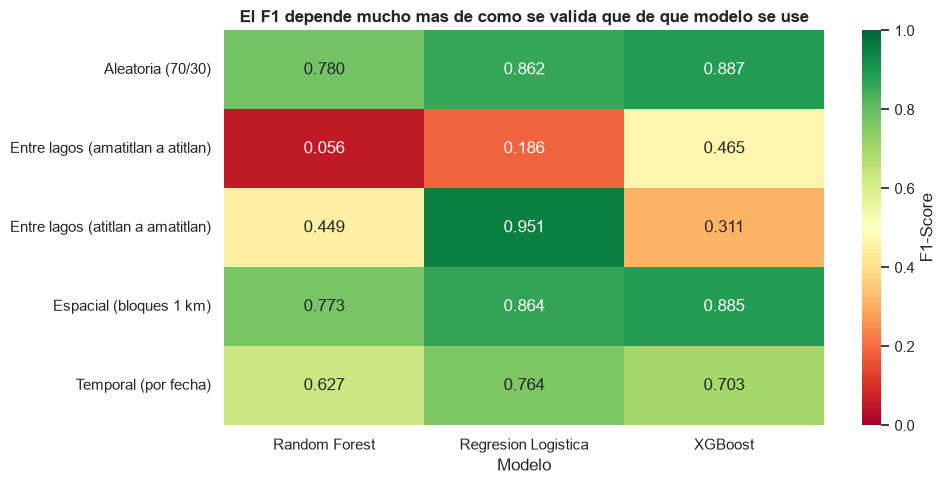
\includegraphics[width=0.75\textwidth]{heatmap_f1_estrategias.png}
    \caption{F1-Score de cada modelo bajo cada estrategia de validación y escenario de generalización.}
    \label{fig:heatmap_f1}
\end{figure}

\subsection{¿Tiene el modelo capacidad suficiente para apoyar el monitoreo?}

\textbf{Sí en Amatitlán, con reservas en Atitlán, y en ningún caso como emisor automático de alertas sin supervisión.}

\begin{itemize}
    \item \textbf{Amatitlán:} XGBoost llega a F1 = 0.9527 con Recall = 0.9745 dentro del lago, y el mapa de 2026-06-19 reproduce la extensión real de la floración con Recall = 0.9981.
    \item \textbf{Atitlán:} Recall = 0.9137 pero precisión = 0.5020, es decir, la mitad de las alertas serían falsas. Sirve como filtro para decidir dónde priorizar el muestreo físico (reduce 287{,}610 píxeles a unos 5{,}000 candidatos), pero no como aviso público sin verificación humana.
    \item \textbf{Entre lagos:} XGBoost, el mejor modelo dentro de un lago, es el peor transfiriendo (F1 = 0.3114), mientras que la Regresión Logística alcanza F1 = 0.9510 en esa misma dirección. No se puede soltar un modelo en un lago nuevo sin verificar su desempeño ahí primero.
    \item \textbf{En el tiempo:} F1 = 0.7031 promediando los folds cronológicos contra 0.8874 con división aleatoria, y tan solo 0.3880 en el peor fold. Ese 0.70 es el techo de desempeño realista para un sistema que predice el futuro.
\end{itemize}

La conclusión metodológica más importante de este laboratorio es que \textbf{la diferencia entre estrategias de validación es mayor que la diferencia entre modelos}: el F1 de XGBoost se mueve entre 0.3114 (transferencia entre lagos) y 0.8874 (división aleatoria), un rango mucho más amplio que el que separa a los tres algoritmos bajo una misma validación. Haberse quedado solo con la división aleatoria habría dado una impresión bastante más optimista -- y menos honesta -- de lo que este modelo puede realmente hacer.

\subsection{Limitaciones}

\begin{itemize}
    \item \textbf{La etiqueta no es una medición de campo.} Sale de umbralizar una clorofila estimada por NDCI, nunca contrastada contra un laboratorio. En el fondo, se entrenó un modelo para reproducir otro modelo, heredando todos sus errores de calibración. Es la limitación de fondo de todo el ejercicio.
    \item \textbf{Pocas fechas:} 19 fechas distintas útiles, folds temporales de apenas tres fechas cada uno, y un fold con solo 86 píxeles positivos de 24{,}436.
    \item \textbf{Resolución de 20 metros:} los errores se concentran donde un solo píxel mezcla agua, vegetación ribereña y fondo somero; las floraciones incipientes o muy pequeñas no son resolubles a esta escala.
    \item \textbf{Sesgo estacional en la muestra:} las escenas más nubladas se descartan, y tienden a concentrarse en la época lluviosa, justo cuando hay más arrastre de nutrientes hacia el lago.
    \item \textbf{Desbalance extremo en Atitlán:} con 0.21\,\% de positivos, la precisión de cualquier modelo queda estructuralmente castigada en ese lago.
    \item \textbf{Coordenadas entre los predictores:} \texttt{y\_utm} se llevó el 63\,\% de la ganancia del modelo actuando como identificador de lago, y removerla no costó desempeño -- no debieron incluirse en un modelo multi-lago desde el principio.
    \item \textbf{Los modelos de árboles no extrapolan:} ante reflectancias fuera del rango visto en entrenamiento (como al transferir de Atitlán a Amatitlán), Random Forest y XGBoost fallan silenciosamente, sin ninguna señal de alerta.
\end{itemize}

\subsection{Qué información adicional mejoraría el modelo}

\begin{itemize}
    \item \textbf{Datos de campo:} muestreos de clorofila y conteo celular que permitan calibrar el NDCI localmente y validar la etiqueta contra una medición real. Es lo que más aportaría, porque ataca la limitación de fondo del ejercicio.
    \item \textbf{Variables meteorológicas:} temperatura del aire, precipitación acumulada previa y viento. Las floraciones responden a agua caliente, superficie calmada y pulsos de nutrientes después de las lluvias, información que no está contenida en la imagen satelital del día. El enunciado del laboratorio sugiere las series históricas de WeatherSpark para ambos lagos como punto de partida.
    \item \textbf{Temperatura superficial del agua}, obtenible del infrarrojo térmico de Landsat 8 y 9, uno de los mejores predictores de floraciones reportados en la literatura.
    \item \textbf{Historia reciente del píxel:} el estado de la escena anterior en el mismo punto, una variable disponible de forma natural en un sistema de monitoreo operativo real.
    \item \textbf{Más escenas}, filtrando por píxel válido en lugar de descartar la fecha completa cuando hay nubosidad parcial, para recuperar imágenes hoy excluidas.
    \item \textbf{Batimetría y uso del suelo de la cuenca}, que ayudarían a explicar dónde se acumula la biomasa y de dónde proviene la carga de nutrientes.
\end{itemize}

% ======================================================================
\section*{Referencias}
\addcontentsline{toc}{section}{Referencias}
% ======================================================================

\begin{itemize}
    \item World Health Organization (2021). \emph{Guidelines on Recreational Water Quality, Volume 1: Coastal and Fresh Waters}, Capítulo 5 (Harmful Algal Blooms) -- Alert Level Framework. \url{https://www.ncbi.nlm.nih.gov/books/NBK572625/}
    \item Chorus, I. \& Welker, M. (eds.) (2021). \emph{Toxic Cyanobacteria in Water}, 2\textsuperscript{a} ed. WHO / CRC Press.
    \item Sentinel Hub -- Repositorio de \emph{custom scripts}, \emph{Cyano Detection Script} (\texttt{cyanobacteria\_chla\_ndci\_l1c}). \url{https://custom-scripts.sentinel-hub.com}
    \item Chen, T. \& Guestrin, C. (2016). XGBoost: A Scalable Tree Boosting System. \emph{Proceedings of the 22nd ACM SIGKDD International Conference on Knowledge Discovery and Data Mining}.
    \item Lundberg, S. M. \& Lee, S.-I. (2017). A Unified Approach to Interpreting Model Predictions (SHAP). \emph{Advances in Neural Information Processing Systems 30}.
    \item Roberts, D. R. et al. (2017). Cross-validation strategies for data with temporal, spatial, hierarchical, or phylogenetic structure. \emph{Ecography}, 40(8).
    \item Laboratorio 4, Parte 2. Análisis de modelos usando datos geoespaciales. CC3084 -- Data Science, Universidad del Valle de Guatemala, Semestre II 2026.
\end{itemize}

\end{document}
